\subsection{Clustering Minimal Description Length}
\label{ssc:mdl-clust}

In this section we analyze changes in the LM minimal description length values
when it is computed for a collection of clusters of arbitrary dimension and size
-- clustering.

For our experiments we performed clustering of the climate dataset,
see Section \ref{ssc:climate}. We performed multiple clusterings of the dataset
varying only one parameter -- \emph{best\_bound}. This parameter affect
cluster partitioning mechanism in LMCLUS algorithm which influence a final
number of generated clusters \cite{Haralick:2007rt}. We generate a sample
composed of clusterings produced by changing \emph{best\_bound} parameter in
range [0.1, 1.2] with value increment of 0.05. This results in 23 clusterings
per each clustering sample. For a statistical evaluation, we collected 1000
clustering sample, total 23000 clusterings.

For the reference to the K{\"o}ppen-Geiger (KG) climate classification system that
identifies 34 climate classes, we set \emph{number\_of\_clusters} parameter,
an expected number of clusters for the LMCLUS algorithm, to 34.
This parameter affects sampling procedure for a manifold basis of a prospective
cluster \cite{Haralick:2007rt}.

In our experiments, we also set minimum cluster size parameter,
\emph{min\_cluster\_size}, to 150, and sampling factor parameter,
\emph{sampling\_factor}, which is used in the sampling heuristics to constrain
a number of samples for potential cluster linear manifold, to 1.0.
Rest of the LMCLUS algorithm parameters where set to default values.
For more detailed description of LMCLUS algorithm parameters consult
Table~\ref{tab:lmclus-params} in the Appendix~\ref{ssec:lmclus-params}.

% Setup



\subsubsection{Parameters of Clusterings}
\label{sssc:clust-params}

We analyzed a clustering size, which is a number of clusters in the clustering,
gathered from generated clustering samples. First, we group all clusterings by
their sizes with respect to \emph{best\_bound} parameter.

\begin{figure}[H]
\center
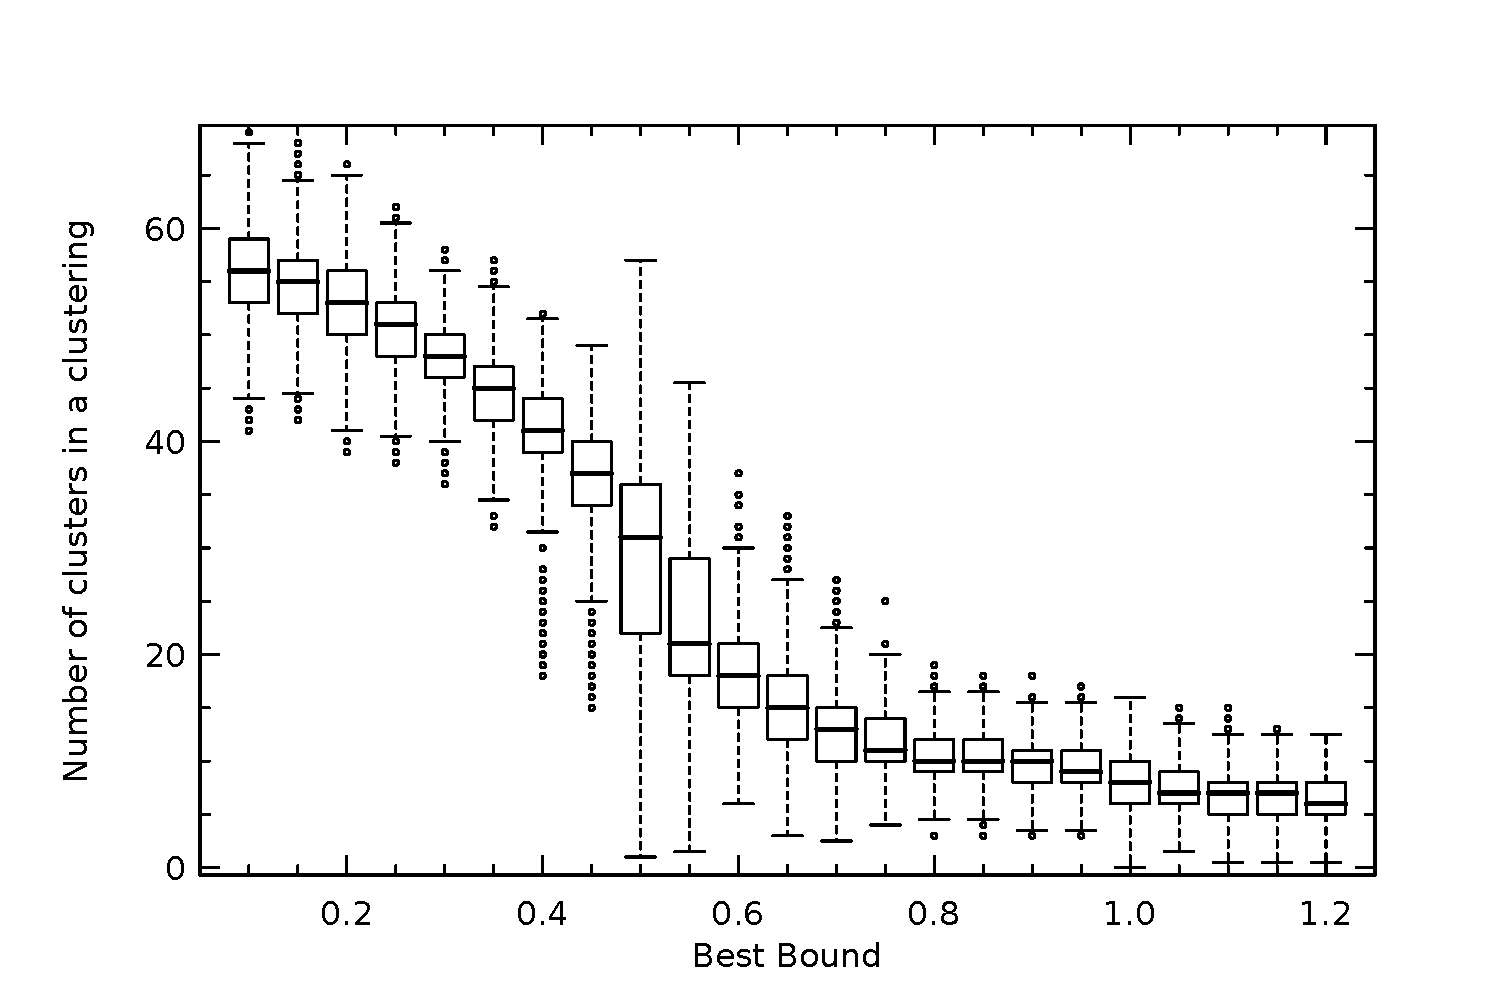
\includegraphics[width=5.5in]{img/mdl-clust_best-bound-cls_1.pdf}
\caption{Size of clusterings (number of clusters in the clustering) produced by LMCLUS algorithm by varying \emph{best\_bound} parameter value.}
\label{fig:best-bound-cls}
\end{figure}



Figure~\ref{fig:best-bound-cls} shows a large variation for clustering sizes
for \emph{best\_bound} in range [0.4,0.7]. This range behaves as a transition
zone between clusterings with a small number of clusters, corresponding to
the large \emph{best\_bound} value, and a large number of clusters,
corresponding to the small \emph{best\_bound} value. We can speculate that for
current dataset algorithm is not able to pick mid range clusters, resulting
in arbitrary partitioning of some large clusters.

\begin{figure}[H]
\center
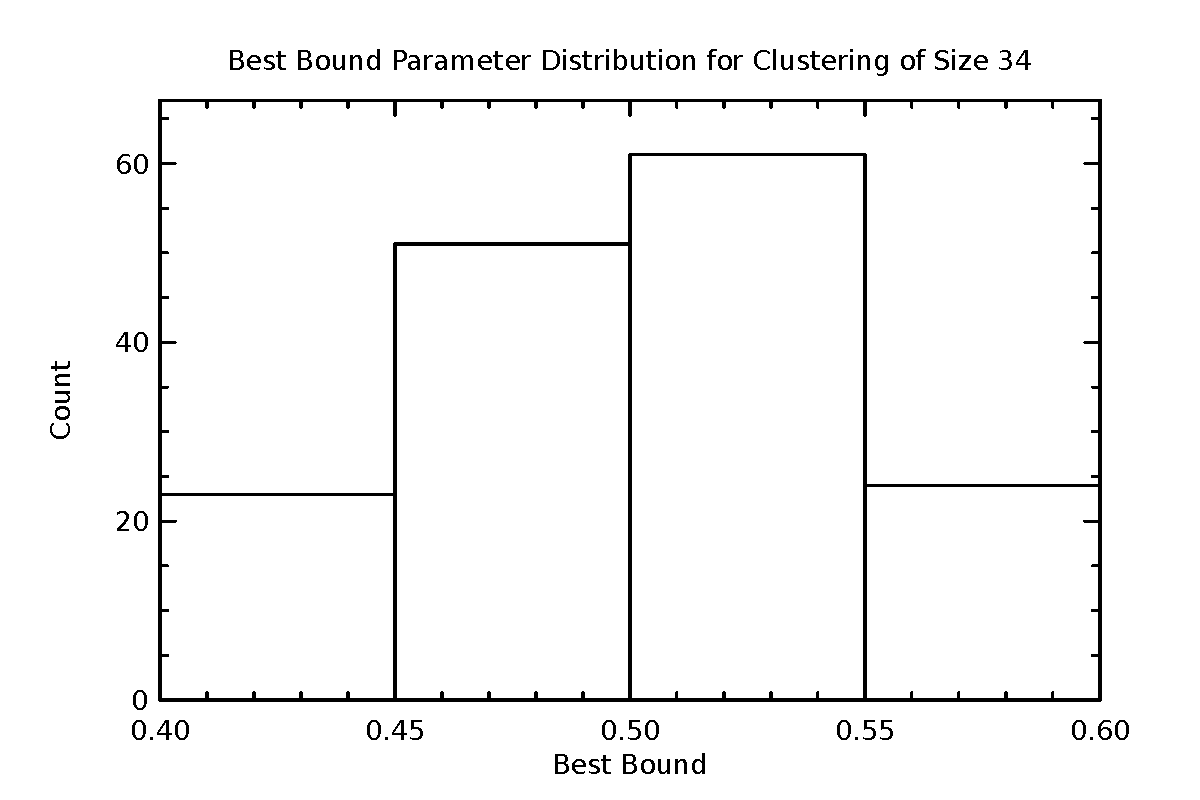
\includegraphics[width=4.5in]{img/mdl-clust_best-bound-cl-34_1.pdf}
\caption{The \emph{best\_bound} parameter value distribution of clustering of size 34.}
\label{fig:best-bound-cl-34}
\end{figure}



Figure~\ref{fig:best-bound-cl-34} shows a distribution of the \emph{best\_bound}
parameter for the clustering size equal to 34, which correspond to the number of
climate zones in K{\"o}ppen-Geiger classification. We can observe that
\emph{best\_bound} parameter is distributed within a "transitional" range where
the clustering algorithm produces clusterings with wide variation of sizes for
given parameters, see Figure~\ref{fig:best-bound-cls}.


Next, we analyze dimensionality of clusters from the sampled clusterings.
Results showed that majority of the clusters in various sized clusterings are
1-dimensional. Usually, the last cluster has dimension zero which is by design -
this cluster is a collection of all outliers that algorithm wasn't able to
associate with any known cluster.
Moreover, a cluster, before last one in a clustering of any size,
has higher dimension then one. This behavior can be attributed to constrained
minimal cluster size, forcing algorithm to generate high-dimensional clusters
with that would pass minimal cluster size threshold, see discussion in
the beginning of Section~\ref{ssc:mdl-clust}.

\begin{figure}[H]
\center
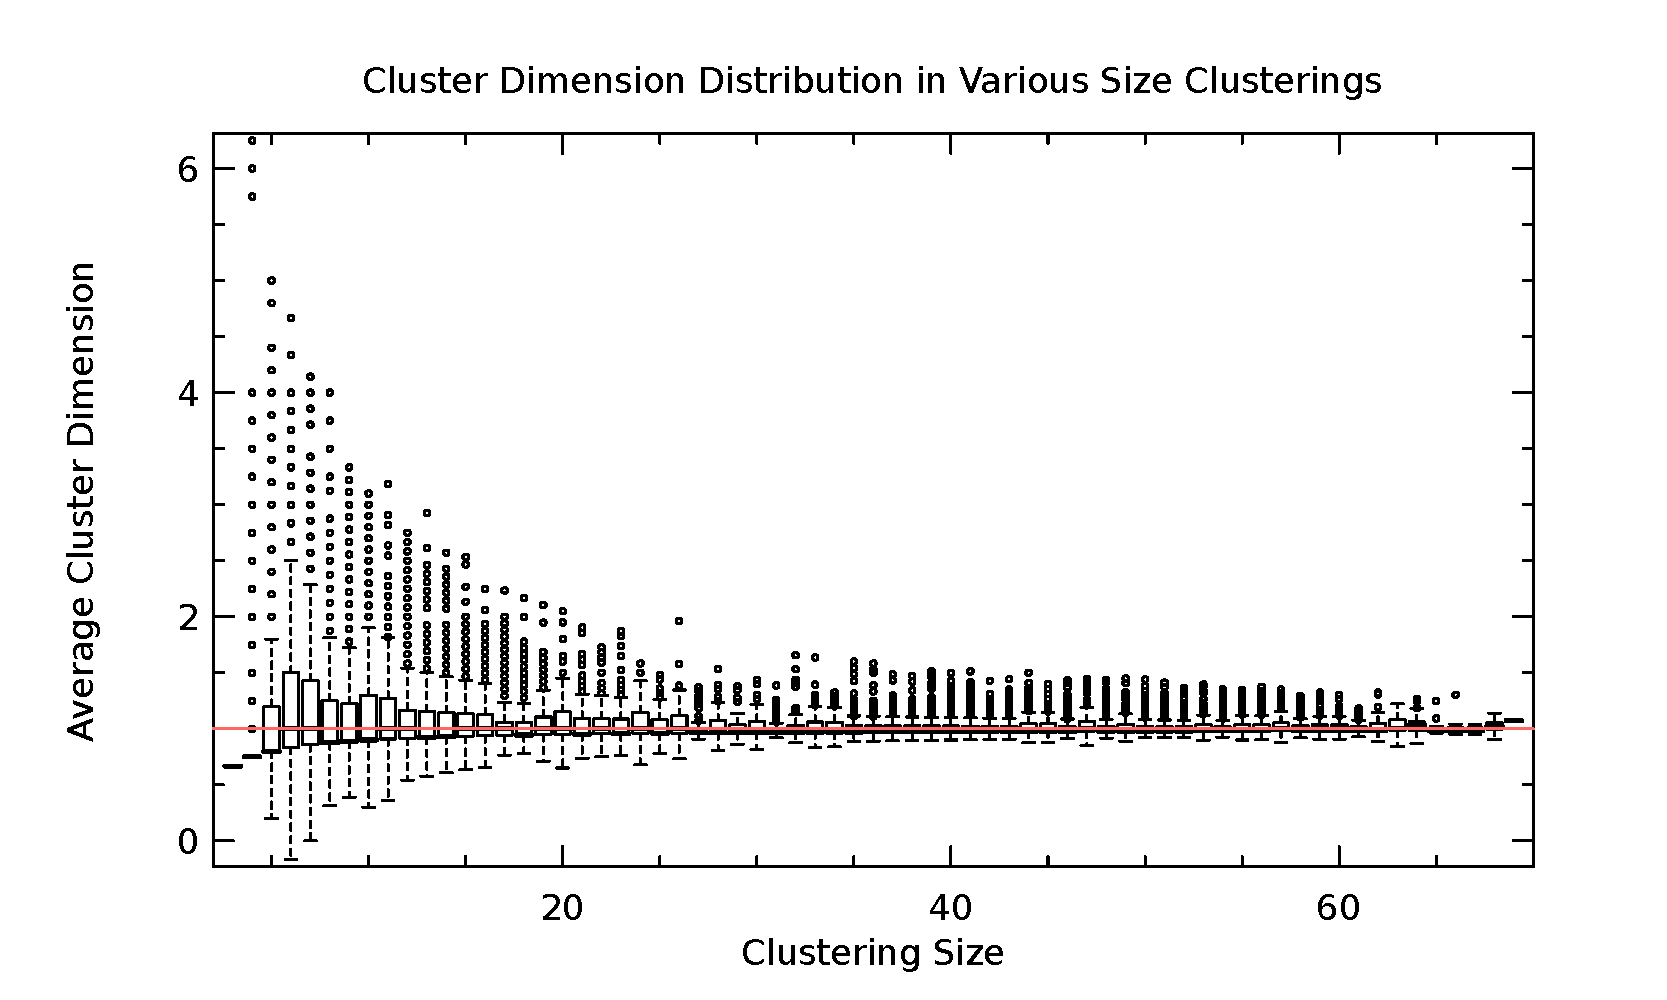
\includegraphics[width=6.0in]{img/mdl-clust_mdl-clust-cdim_1.pdf}
\caption{The \emph{best\_bound} parameter value distribution of clustering of size 34.}
\label{fig:mdl-clust-cdim}
\end{figure}



Figure~\ref{fig:mdl-clust-cdim} shows a cluster dimension distribution for
clusterings of different size. The average dimension of clusters approaches 1
(red line) as number of clusters grows in a clustering. However, there is
a large variability in a cluster dimensionality for small-sized clusterings,
which gradually decreases as the clustering size increases.


In order investigate further occurrence of this pattern, we will look at
the cluster size in generated clusterings. We grouped clusters from
the clusterings of the same size and pooled together corresponded cluster sizes.

\begin{figure}[H]
\center
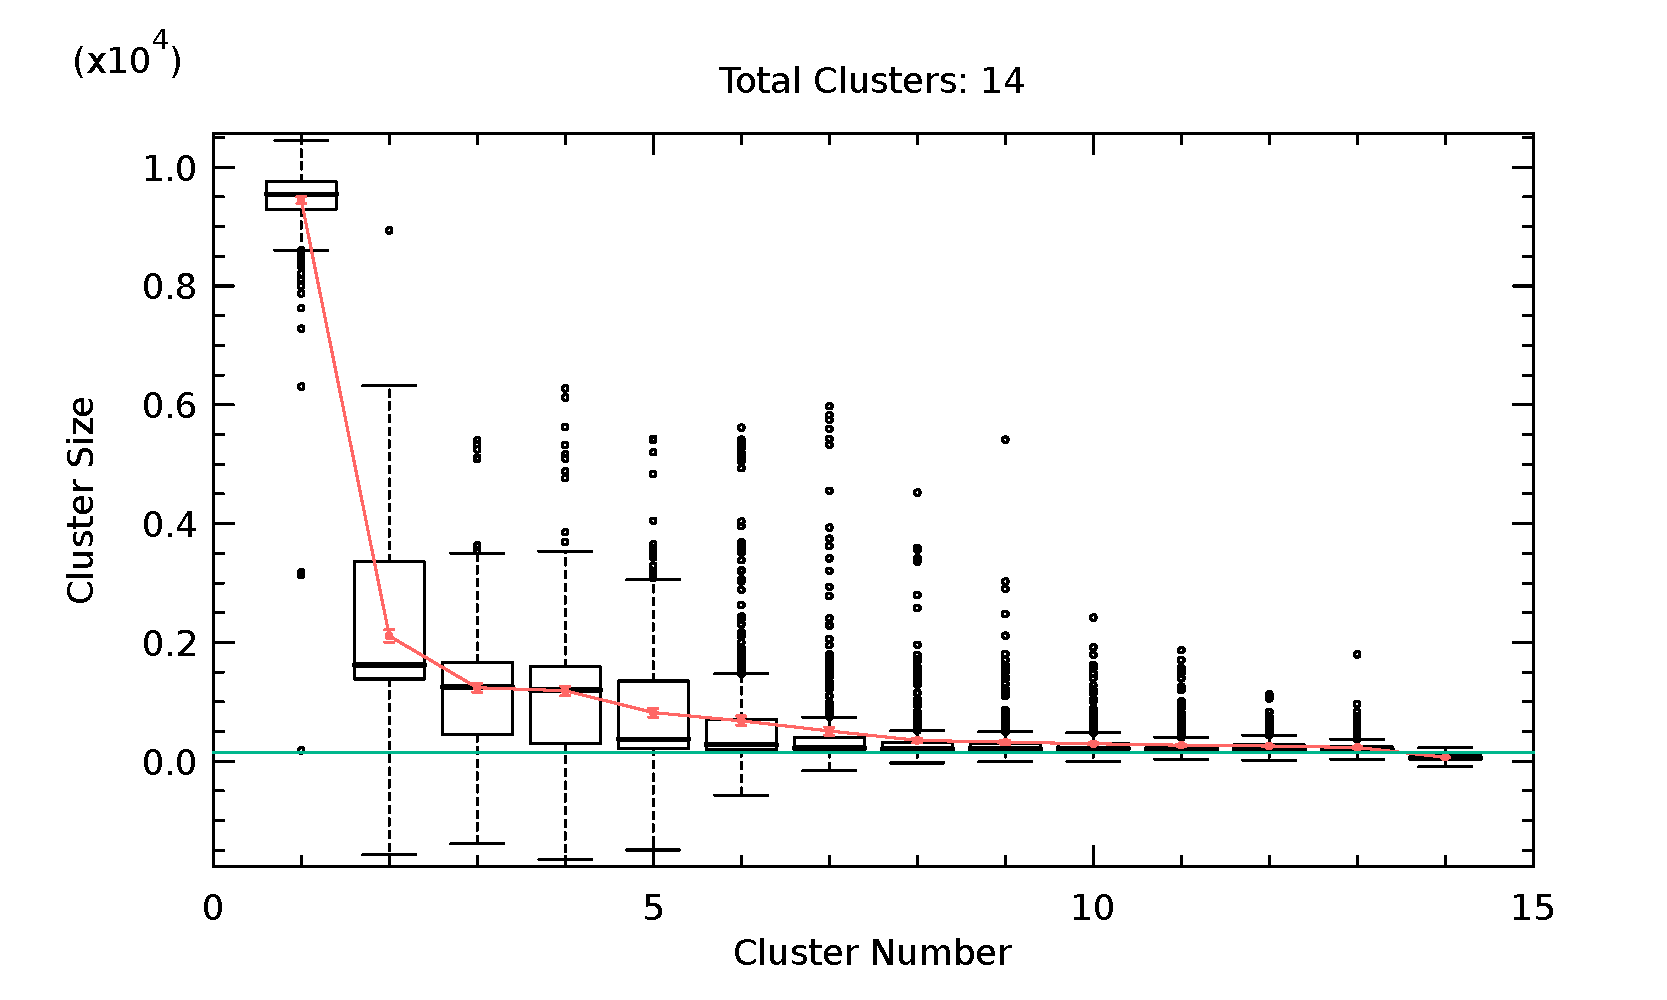
\includegraphics[width=6.0in]{img/mdl-clust_clust-size-14_1.pdf}
\caption{Cluster size distribution for the clustering of size 14.}
\label{fig:clust-size-14}
\end{figure}



Figure~\ref{fig:clust-size-14} shows distribution of the cluster sizes for
clusterings with 14 clusters. The red line on a plot is a bootstrapped mean
cluster size with the corresponding 95\% confidence interval, and the blue line
is a minimal cluster size specified by the LMCLUS parameter,
\emph{min\_cluster\_size}, which is set to 150.

As the number of clusters in the clustering grows, the cluster size  approaches
to the minimal cluster size threshold. Moreover, the cluster size gradually
decreases, for from large clusters, generated at the beginning of
the clustering procedure, to the clusters with the size near the threshold limit
for clusters produced near the end of clustering procedure. This behavior is
observed for all sizes of clusterings, especially with few clusters.


\subsubsection{Clustering MDL Calculations}
\label{sssc:clust-mdl}

In our calculations of MDL values for clusterings, we used following parameters:
an encoding model constant, $P_m$, set to 32, an encoding data constant,
$P_d$, set to 16, and the user-defined quantization error upper boundary,
$\varepsilon$, set to 0.001.




In two-part MDL calculation for linear manifold clusters, first part, a cluster
model description is computed by \eqref{eq:mdl-lmc-model},
$L(\mathcal{M}) = P_m N (N+1)/2$.
However, when cluster is not of a linear manifold form, we calculate its
description as if it's a spherical cluster. Thus, we only need to encode center
of the spherical cluster in a model description, $L(\mathcal{M}) = P_m N$.

\begin{figure}[H]
\center
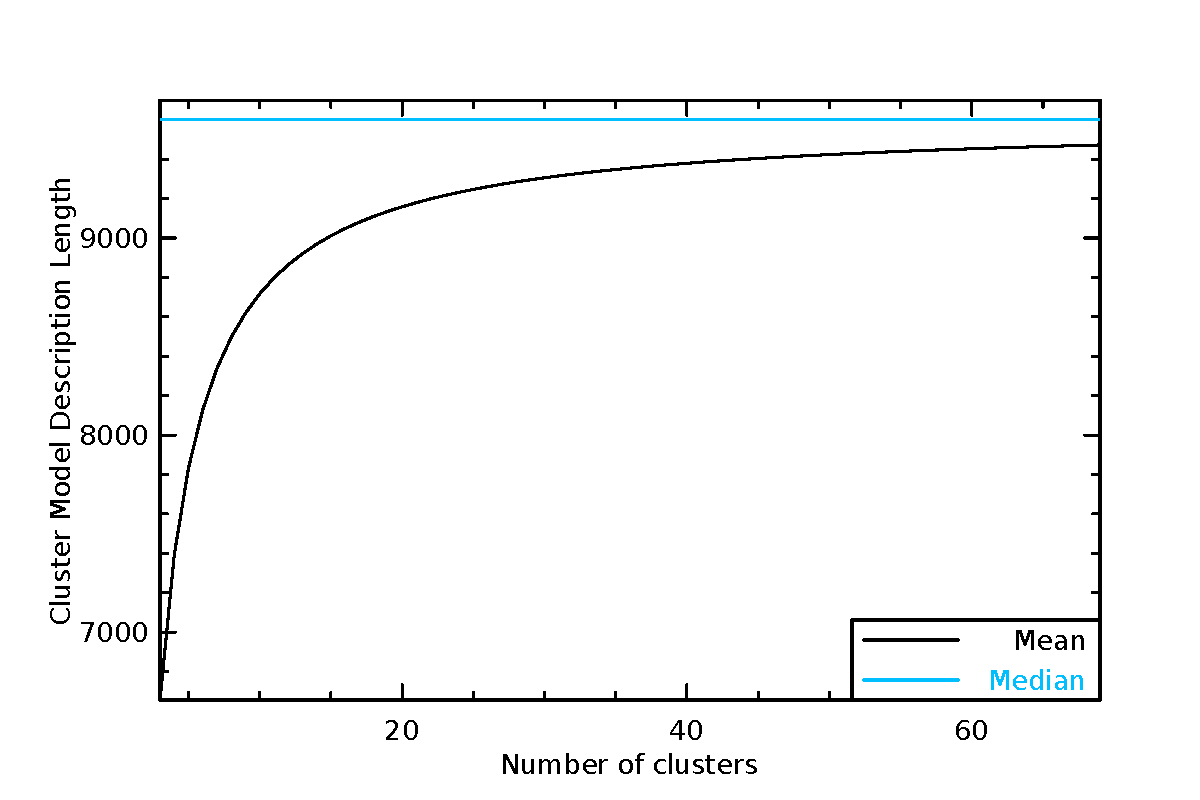
\includegraphics[width=5.0in]{img/mdl-clust_model-dl-stats_1.pdf}
\caption{Cluster model description length mean amd median values.}
\label{fig:model-dl-stats}
\end{figure}



Figure~\ref{fig:model-dl-stats} shows mean and median model description length
values for sampled clusterings grouped by their size. The model MDL for
1-dimensional LM cluster is 32 x 24 x 25/2 = 9600. As expected, a median MDL for
a clusters in sampled clusterings is 9600 bits, which corresponds to MDL value
of the dominant cluster in all generated clustering samples. A mean cluster
model MDL value is expected to approach median value. As almost every clustering
contains a 0-dimension cluster of outliers, the more clusters in the clustering,
the closer average model MDL value to the model MDL of 1-dimensional LM cluster.

In context of the MDL calculation for a clustering, the total model MDL of
a clustering $\mathcal{K}$, composed of $k$ clusters, is calculated as

$$L(\mathcal{K}) = \sum_k L(\mathcal{M}_k)$$

Thus, we should expect linear grows of the clustering model MDL value with
a number of clusters, because every cluster has only one 0-dimensional "noise"
cluster and the rest of the clusters are described by constant number of bits,
see Figure~\ref{fig:clustering-model-dl}.

\begin{figure}[H]
\center
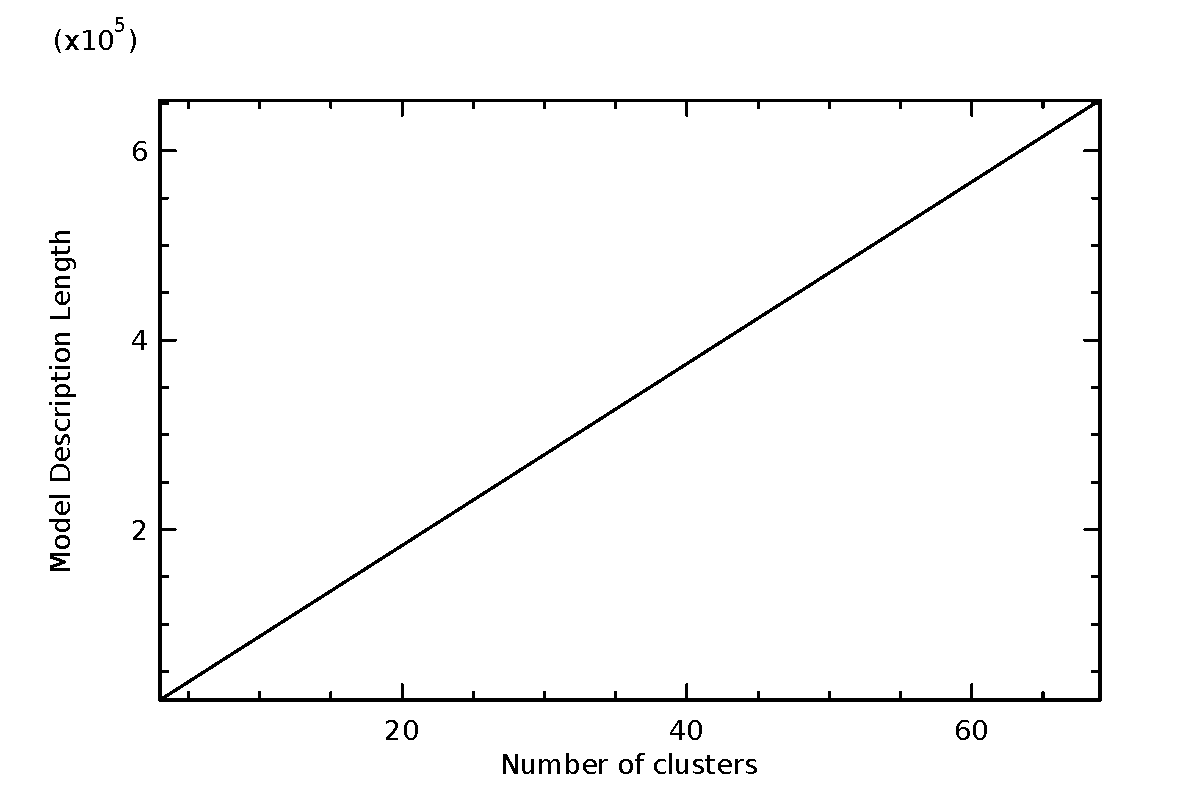
\includegraphics[width=4.0in]{img/mdl-clust_clustering-model-dl_1.pdf}
\caption{Clustering Model Description Length.}
\label{fig:clustering-model-dl}
\end{figure}



In context of the MDL calculation for a clustering, a total data MDL value of
a clustering $\mathcal{K}$, composed of $k$ clusters, is calculated as

\begin{equation}
L(D \;|\;\mathcal{K}) = \sum_k L(\mathcal{C_k} \;|\;\mathcal{M_k}) = \sum_k P_d M_k J_k + \sum_k J_k S_{k, M_k}(\varepsilon)
\end{equation}

where $L(\mathcal{C} \;|\;\mathcal{M})$ is a description length of the cluster
$\mathcal{C}$ encoded given the model $\mathcal{M}$, see \eqref{eq:mdl-lmc-data}.




If size of the dataset $D$ is $d = |D| = \sum_k J_k$, then first term,
$\sum_k P_d M_k J_k$ can be approximated with $(P_d d) E[M]$,
where $E[M]$ is an expected value of the cluster dimensionality in a particular
clustering, and $d = \sum_k J_k$ is a size of the dataset.
Second term, $\sum_k J_k S_{k, M_k}$ can be views as expected values of
the entropy of the OSC points distribution $(d)E[S]$, so

$$L(D \;|\;\mathcal{K}) = (P_d d) E[M] + (d) E[S]$$

We also would like to compare data MDL of the clustering when all components are
just encoded with entropy, as in case of MDL calculation for a zero-dimensional
cluster.

$$L_z(D \;|\;\mathcal{K}) = (d)E[S]$$

Figure~\ref{fig:clustering-data-dl} shows a distribution of the clustering data
MDL values, $L(D \;|\;\mathcal{K})$, as a box plot, and bootstrapped mean value
of $L(D \;|\;\mathcal{K})$, as well as bootstrapped mean value of a clustering
entropy from all components of the cluster points, $L_z(D \;|\;\mathcal{K})$.

\begin{figure}[H]
\center
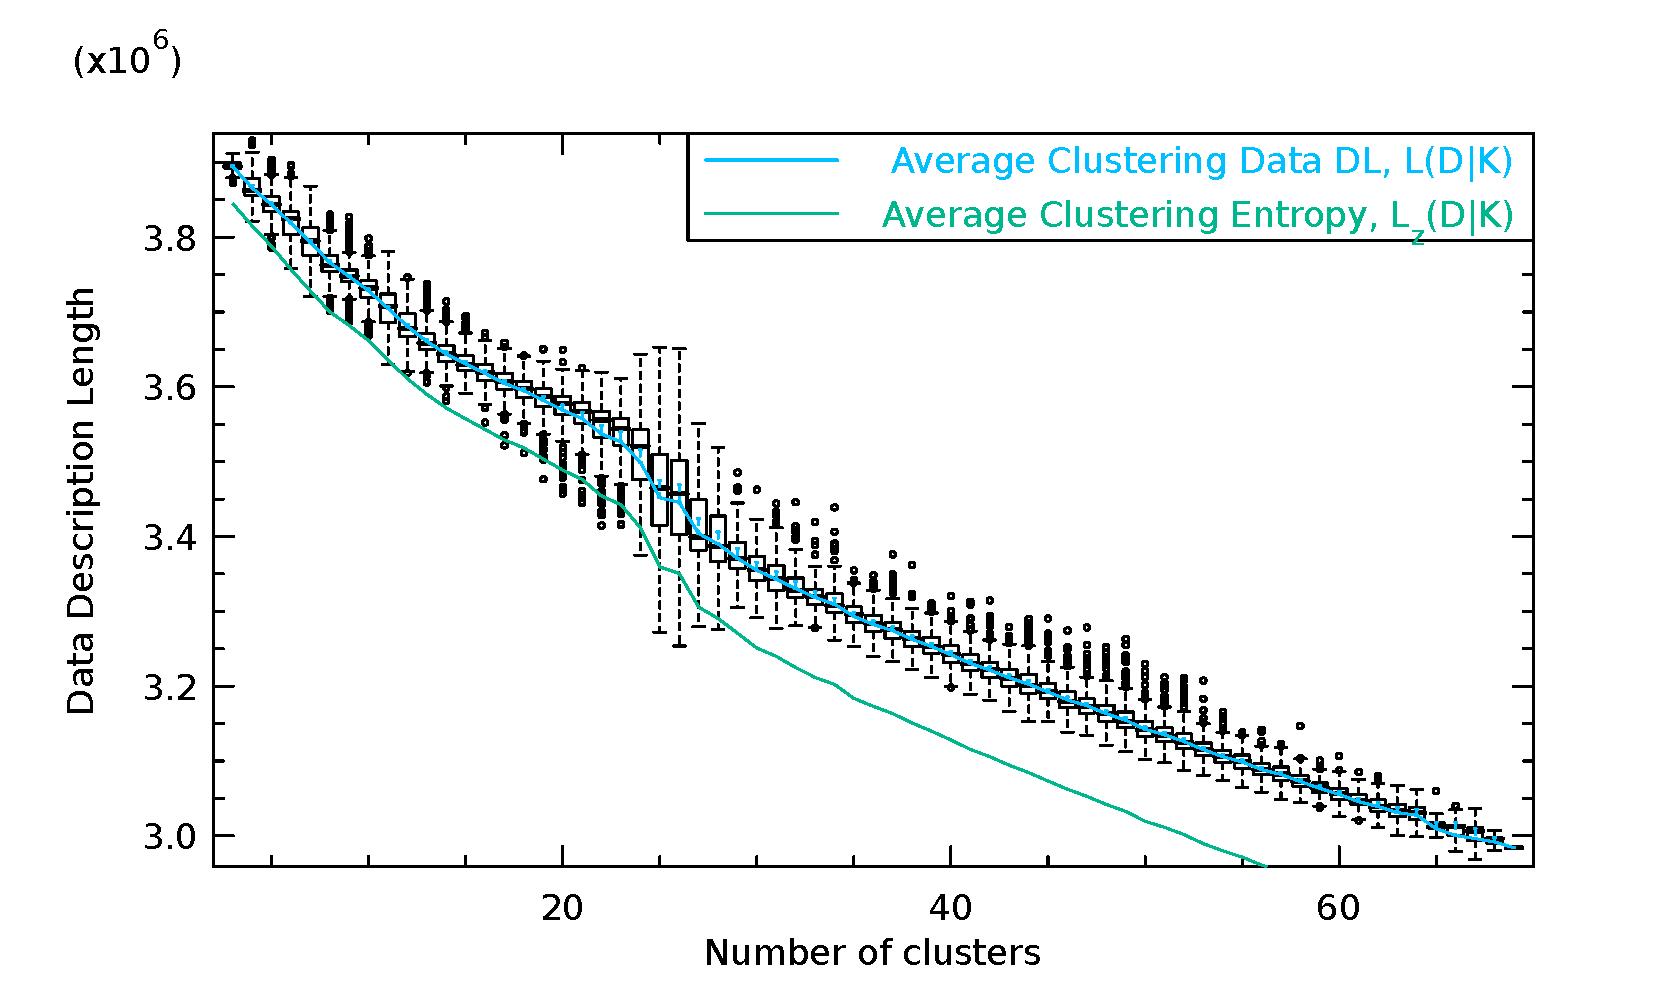
\includegraphics[width=5.0in]{img/mdl-clust_clustering-data-dl_1.pdf}
\caption{Clustering Data Description Length.}
\label{fig:clustering-data-dl}
\end{figure}



Displayed pattern shows expected linear downward trend: when the number of
clusters increases in the clustering, the clustering MDL value tend to decrease.
This happens because clusters become more compact and encoding is better for
such clusters yielding smaller MDL value. There is only one discrepancy in
the clustering size interval of [20,30]. It can be attributed to large cluster
dimensionality variation for clustering with particular number of clusters.

Now, we can calculate clustering MDL for the dataset $D$ by combining two parts:
$L(\mathcal{K})$ and $L(D \;|\;\mathcal{K})$.
We predicted that with that two-parted linear manifold MDL, we would have
large MDL value when the clustering has few clusters, which is driven by large
\emph{data}-part of joint MDL value for small-sized clusterings,
as well as large MDL value when the clustering has many clusters, which is
driven by large \emph{model}-part MDL value for large-sized clusterings.
Between these MDL value extrema, we should have clustering with minimal MDL
value characterized by balancing model and data MDL parts.

\begin{figure}[H]
\center
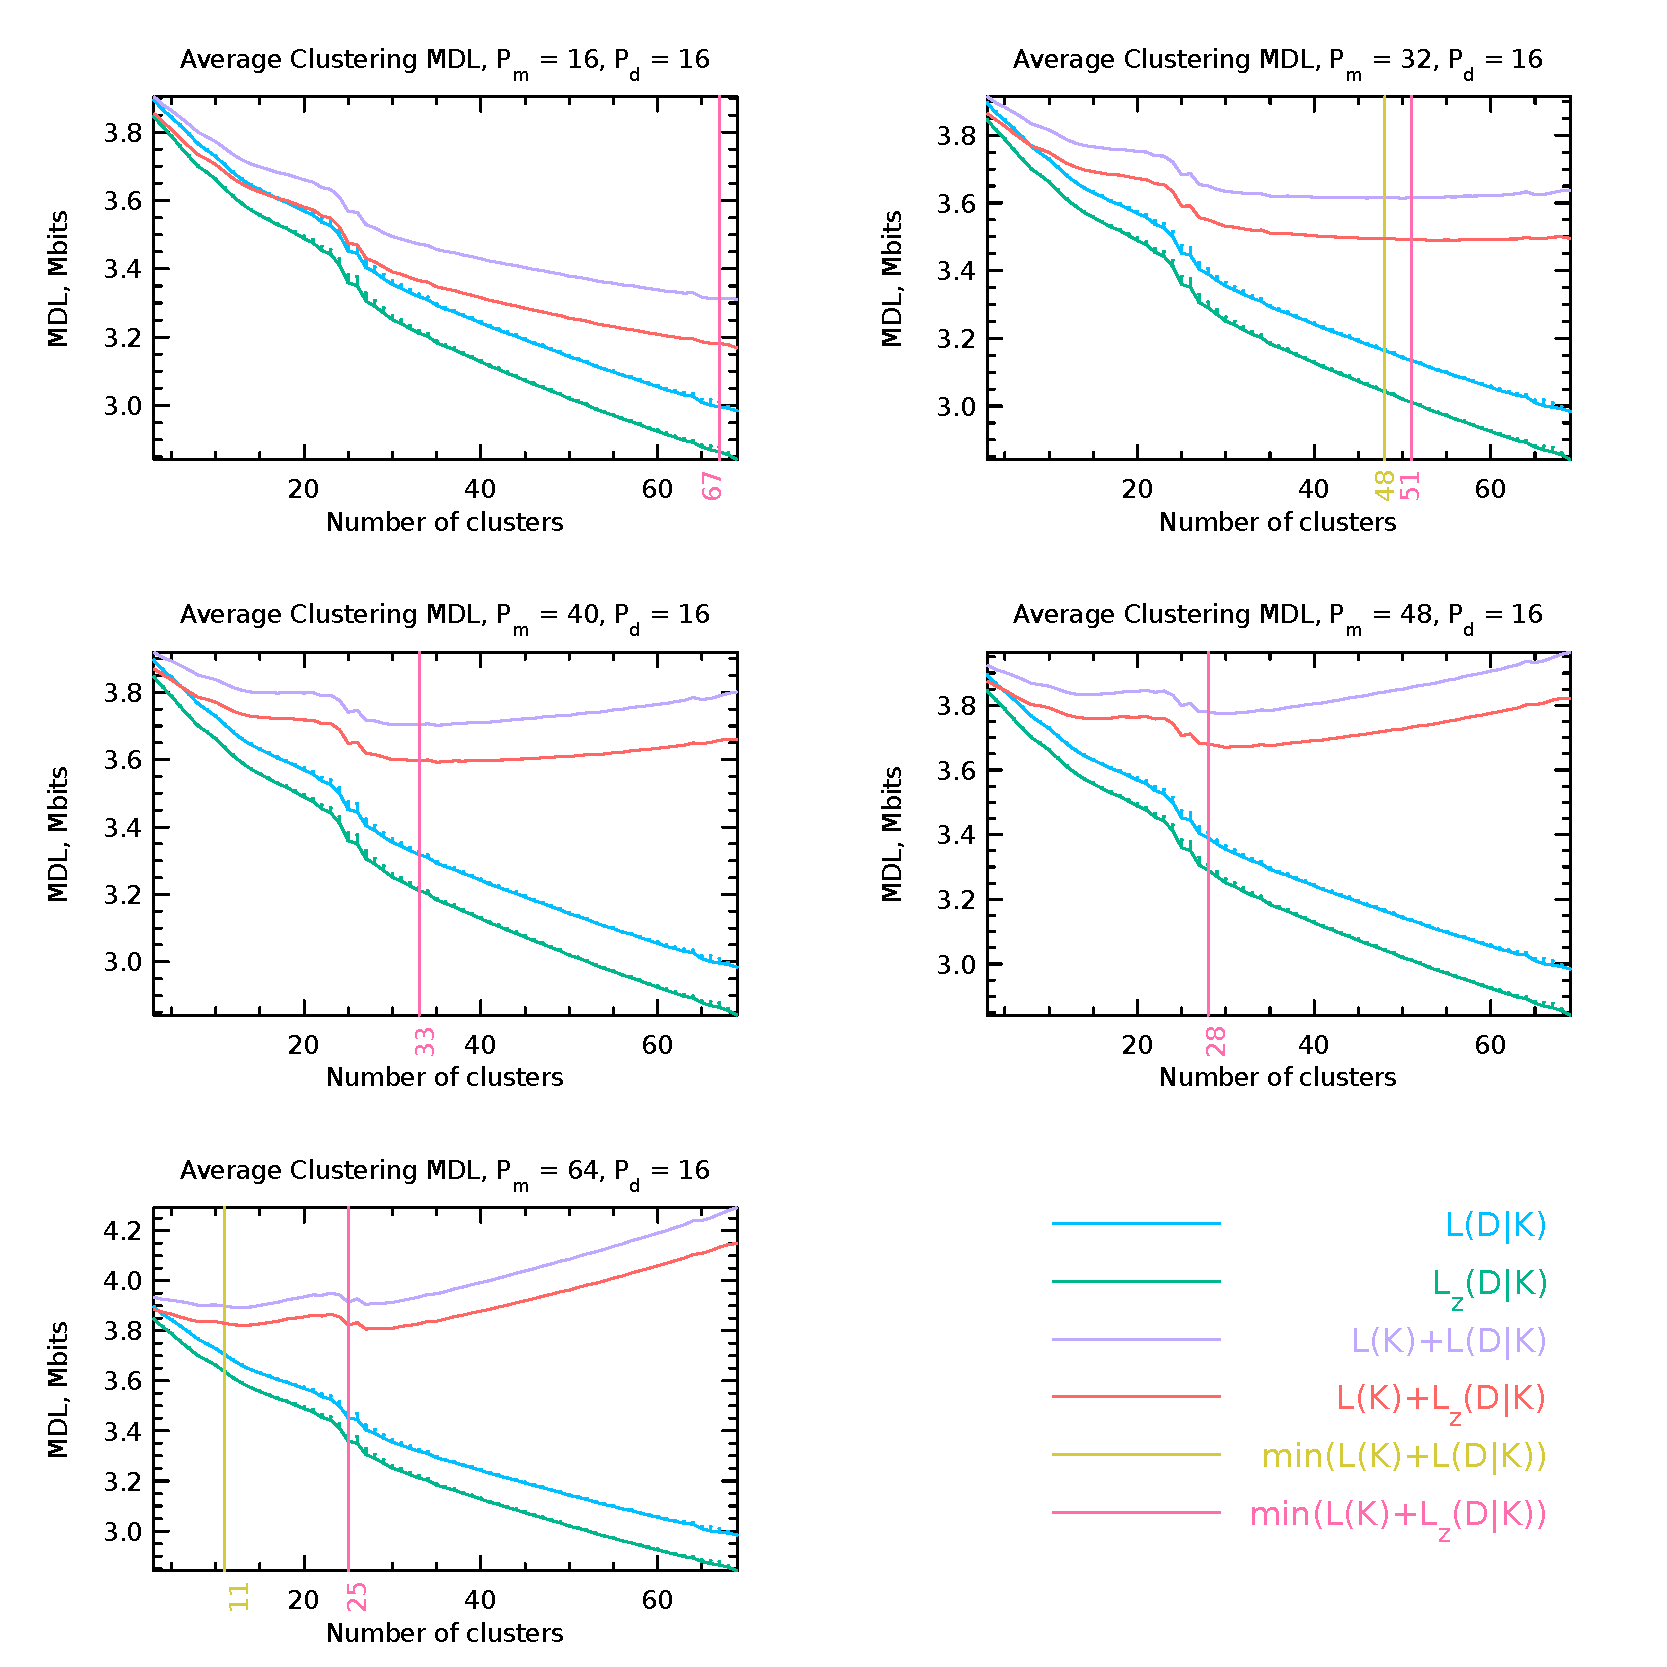
\includegraphics[width=5.0in]{img/mdl-clust_clustering-mdl_1.pdf}
\caption{Avarage Clustering MDL for different encoding constant values.}
\label{fig:clustering-mdl}
\end{figure}



Figure~\ref{fig:clustering-mdl} shows plots of average two-part MDL values and
data MDL values (as well as MDL value based on cluster entropy) for clusterings
of different size. Vertical lines on plots identify clustering sizes which are
corresponded to the minimal MDL value under particular parameters.
We generated these plots for various $P_m$ constants, in order to see how these
constant would affect total MDL value, as it is primary parameter for the model
MDL calculation.

We found that with default parameters $P_m = 32$ and $P_d = 16$, the clustering
MDL value levels on after clustering size 30, reaching minimum value for
the clustering with 51 cluster and then gradually increases. With $P_m < 32$,
the clustering MDL value continues to decrease and we are not able to determine
correctly minimal MDL as we have a little or no data for clustering size beyond
67 clusters. With $P_m > 32$, we could clearly identify the minimal MDL value
and see its increase as clustering size grows.

Notably, $P_m = 40$ lands minimum clustering MDL for clusterings with
33 clusters which is very close to the expected value of 34 climate classes from
the K{\"o}ppen-Geiger (KG) climate classification.

\begin{figure}[H]
\center
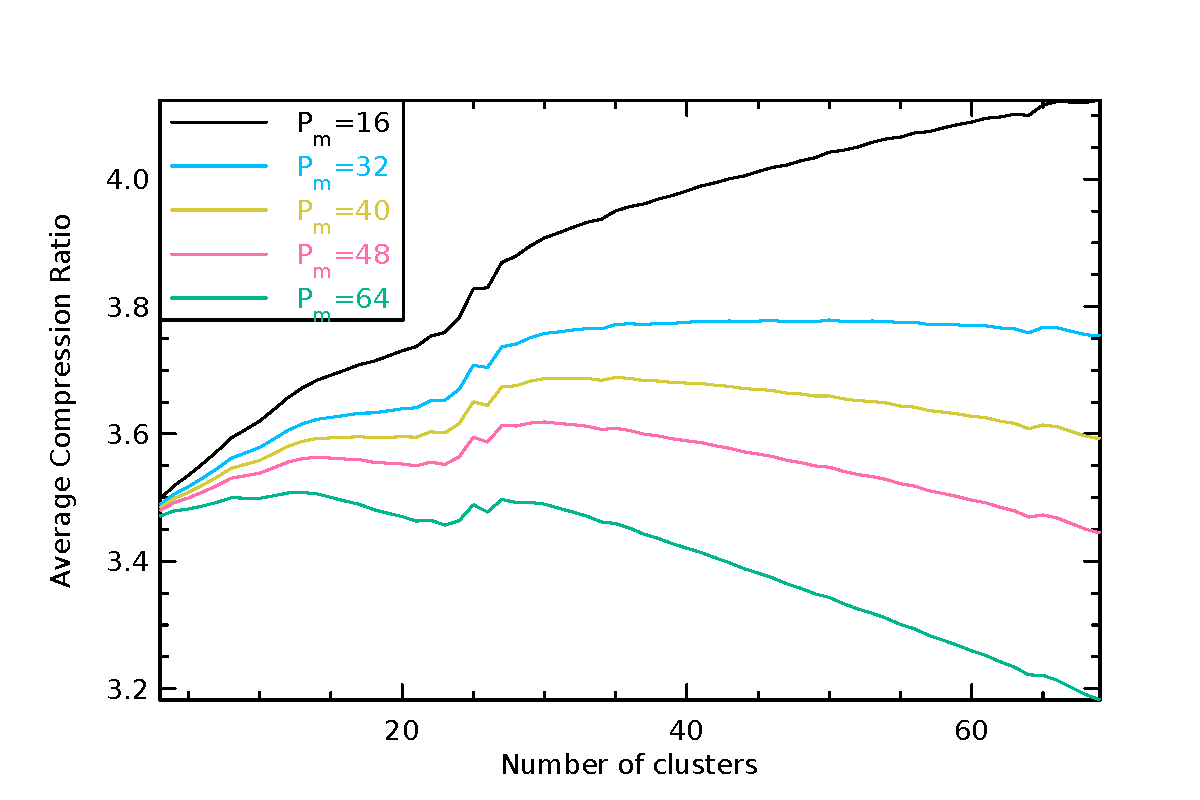
\includegraphics[width=5.0in]{img/mdl-clust_clustering-mdl-cr_1.pdf}
\caption{Average clustering MDL compression ratio.}
\label{fig:clustering-mdl-cr}
\end{figure}



Figure~\ref{fig:clustering-mdl-cr} shows average compression ration calulated
for various model encoding constants.
Using average clustering MDL, we can evaluate some of the parameters of
the MDL heuristics for LMCLUS algorithm such as the encoding constants,
$P_d$ and $P_m$, and the compression ratio. Compression ratio defines the ratio
between an uncompressed (raw) encoding of the dataset with constant precision,
$P_r$ and a clustering MDL  which is an encoding of the dataset using
a particular clustering partition. It's calculated as follows
$$CR = \frac{P_rNd}{MDL}$$
where $P_r = 32$ is a precision encoding constant for raw data, $N$ is dataset dimension, and $d$ is a size of the dataset.
